% !TEX program = xelatex
% main.tex — arXiv preprint, 繁體中文版（XeLaTeX 編譯）
% Compile: xelatex main && bibtex main && xelatex main && xelatex main
%      或: latexmk -xelatex main

\documentclass[UTF8,fontset=none,10pt,a4paper,twocolumn]{ctexart}

% ---- 繁體中文字體（Windows 內建）-------------------------------------
\setCJKmainfont[BoldFont={Microsoft JhengHei Bold},ItalicFont={PMingLiU}]{PMingLiU}
\setCJKsansfont{Microsoft JhengHei}
\setCJKmonofont{PMingLiU}

% ---- Packages ----------------------------------------------------------
\usepackage[a4paper,margin=1in]{geometry}
\usepackage{microtype}
\usepackage{amsmath,amssymb}
\usepackage{booktabs}
\usepackage{tabularx}
\usepackage{array}
\usepackage{multirow}
\usepackage{enumitem}
\usepackage{verbatim}
\usepackage{fancyvrb}
\usepackage{url}
\usepackage{xcolor}
\usepackage{graphicx}
\usepackage{tikz}
\usetikzlibrary{arrows.meta,positioning,shapes.geometric,calc,fit}
\usepackage{caption}
\usepackage{listings}
\usepackage{hyperref}
\hypersetup{
  colorlinks=true,
  linkcolor=blue!50!black,
  citecolor=blue!50!black,
  urlcolor=blue!50!black,
}
\usepackage[capitalize,nameinlink]{cleveref}

\lstset{
  basicstyle=\ttfamily\footnotesize,
  breaklines=true,
  columns=fullflexible,
  showstringspaces=false,
  frame=single,
  framesep=4pt,
  rulecolor=\color{gray!40},
  backgroundcolor=\color{gray!4},
}
\setlist{topsep=2pt,partopsep=0pt,itemsep=2pt,parsep=0pt}

% 雙欄下讓行距彈性化,長 \texttt{} 識別符整個換到下一行而非中斷
\sloppy
\tolerance=2000
\emergencystretch=5em

% ctexart cleveref aliases
\crefname{section}{\S}{\S}
\Crefname{section}{\S}{\S}

% ---- Title -----------------------------------------------------------
\title{LLM API 中轉端點的模型替換偵測：\\
  171 個端點 14 天的測量研究 \\[6pt]
  \large \textit{Measuring Model Substitution in LLM API Resellers:\\
    A 14-Day Study of 171 Endpoints}}

\author{Bazaarlink 研究團隊\\
  \texttt{bazaarlink.ai}\\
  \href{https://github.com/Bazaarlinkorg/LLMprobe-engine}{github.com/Bazaarlinkorg/LLMprobe-engine}}

\date{}

\begin{document}
\maketitle

% =====================================================================
\begin{abstract}
大型語言模型（LLM）API 中轉市場自 2024 年起快速擴張，其成因為上游服務商對特定地區之服務政策限制。由於上游無法認證中轉商實際路由之後端模型，且協定層響應於不同模型間幾乎一致，下游購買者無法直接察覺模型被靜默替換的行為。本論文設計一套四層黑箱偵測系統，每層採用獨立行為指紋通道：表面族別分類器、自我宣告字串歸零的行為對照欄位、子模型確定性匹配（截止日期 / 能力測驗 / 拒絕前綴）、以及涵蓋拒絕梯度、格式偏好、數值不確定性的行為向量擴展層。本研究於 2026-04-12 至 2026-04-25 共 14 日內對 171 個中轉端點累計 625 次探測。在固定樣本的合成壓力測試中，本系統對同家族替換達 94.4\% 真陽性率（$n{=}18$；Wilson 95\% 置信區間 $[74.2\%, 99.0\%]$），對真品 0\% 假陽性率（$n{=}6$）。實地測量結果：\textbf{9.9\% 端點（17/171）呈現至少一次替換事件；嚴格門檻下（樣本 ${\geq}5$、違規率 ${\geq}20\%$）1.3\%（2/149）符合持續性替換候選標準}。本文的核心實證貢獻在於深度案例分析：R1 顯示同一宣稱模型可被動態路由至多個後端，R2 顯示版本標籤會被系統性泛化，R6 則顯示單次事件式替換亦可由內部一致證據鏈捕獲。觀察到的替換可歸納為五大類：跨家族冒充、靜默降級、靜默升級、版本標籤造假、提供商行為注入。本研究與 Liu 等人（arXiv:2604.08407）~\cite{liu2026agent}對 LLM 供應鏈惡意中介者主動安全攻擊的測量互補——後者測量「中轉商主動攻擊使用者」、本論文測量「中轉商替換模型品質」——並提出三項揭露義務政策建議。

\medskip
\noindent\textbf{關鍵詞:} LLM API 中轉; 模型替換; 行為指紋; 消費者保護; 黑箱稽核.
\end{abstract}

% =====================================================================
\section{緒論}\label{sec:intro}

\subsection{由訪問封鎖催生的市場}
Anthropic 與 OpenAI 在其公開的服務條款與可接受使用政策中~\cite{anthropic2026aup,openai2026usage}，對部分國家與地區的服務可用性設有限制；其旗艦產品線在這些受限地區無法直接購買、無法透過官方支付管道計費、亦無法由當地企業以正規票據認列為支出。受限地區的軟體開發者與企業對前沿 LLM 的需求並未因此消失；相反地，生產力工具的競爭壓力反而強化了對這些工具的需求。由此產生的供需缺口，於過去十二個月催生了一個高速成長的中轉產業：第三方營運商於可訪問地區建立 OpenAI 相容 HTTP 端點，背後以官方 API 金鑰向 Anthropic、OpenAI、Google、xAI 等上游服務商發起請求，再以較高的單位價格轉售給受限地區的下游使用者。

此種中轉模式並非 API 經銷商的常見形態。傳統 API 經銷商通常與上游服務商有正式合約、存在合約上的 SLA、其交付的服務在介面上即可被識別來源。而本研究所稱的中轉端點屬於\textbf{未授權之灰色市場}：上游服務商通常並未授權其轉售、其向上游發起的 API 金鑰於上游帳本中無法與下游購買者一一對應、其端點的下游使用者多為被動接受介面相容性即假設服務同質性。

\subsection{信任假設的崩潰}
下游使用者對中轉端點的信任傳統上仰賴四個假設：（1）\textbf{介面假設}——端點實作 OpenAI 相容協定，故其行為與 OpenAI 官方接近；（2）\textbf{自我宣告假設}——在請求中傳入 \texttt{model: claude-opus-4-7} 並收到自我宣告為 Claude 的響應，表示後端確為該模型；（3）\textbf{品牌假設}——端點網站陳列 Anthropic 與 OpenAI logo、客服宣稱「官方代理」者，後端來源即為官方；（4）\textbf{價格假設}——端點不會在收取高階模型費率的同時轉路由到低階模型。本研究將證明上述四個假設在當前中轉市場上全部失效。

\subsection{研究問題}
\textbf{RQ1（普遍性）}：在當前活躍的 LLM API 中轉端點中，有多大比例的端點呈現可被外部觀察者偵測到的模型替換行為？
\textbf{RQ2（型態）}：偽裝行為可被歸納為哪些可重複的模式？
\textbf{RQ3（偵測可行性）}：在僅能透過黑箱 API 觀察的條件下，能否設計出兼具高真陽性率與低假陽性率的偵測方法？
\textbf{RQ4（消費者影響）}：上述偽裝行為對下游使用者構成何種具體傷害？對監管與上游服務商有何政策意涵？

\subsection{研究貢獻與相關工作對位}
本研究的貢獻為：（1）首次系統性的中轉市場替換行為測量；（2）一套四層獨立指紋的可重現黑箱偵測方法論，於固定樣本合成測試中達到 94.4\% 同家族真陽性率與 0\% 假陽性率；（3）替換行為之五大類型分類學；（4）消費者保護視角的政策分析，提出三項可立即實施的揭露義務建議。

\paragraph{與相關工作之對位}
本論文的最近同儕是 Liu 等人~\cite{liu2026agent}，他們對 428 個 LLM API router 進行\emph{主動安全攻擊}之測量——payload 注入、secret/credentials 外洩、規避偵測、加密貨幣盜取等。本研究測量正交軸：router \emph{被動品質替換}——亦即將宣稱提供的高階模型靜默路由至較低階或不同模型——而於使用者系統不施加任何主動入侵行為。兩篇研究合計覆蓋 LLM API 供應鏈之主要威脅面：Liu 等人測量「router 對使用者做了什麼」，本論文測量「router 對模型做了什麼」。

層\textcircled{\scriptsize 4}（\cref{sec:layer4}）的技術構件參考三條既有研究線。拒絕梯度受拒絕方向（refusal direction）之機械可解釋性研究啟發~\cite{arditi2024refusal}。格式指紋根植於「風格偏好為預訓練固化、難以由運行時指令改寫」之觀察~\cite{mcgovern2024stylistic}。校準不確定性通道借用 Kadavath 等人對 LLM 自我認知之圓整率（round-rate）直觀~\cite{kadavath2022know}。層\textcircled{\scriptsize 3}子模型確定性匹配延伸 LLMmap~\cite{pasquini2024llmmap} 之行為指紋方法，但聚焦於同家族內鑑別而非跨家族識別。\cref{sec:policy} 之經濟分析建構於 Akerlof 對「品質不可觀察市場之資訊不對稱」之經典分析~\cite{akerlof1970lemons}。方法論設計參考 Paxson 之網際網路測量穩健性框架~\cite{paxson2004sound}。

% =====================================================================
\section{威脅模型}\label{sec:threat}

\subsection{攻擊者類型}
依商業動機分類：

\begin{itemize}
\item \textbf{套利型 (arbitrage)} 宣稱模型 $M_{\text{high}}$；實際路由至同家族但較低階的 $M_{\text{low}}$（例如宣稱 Opus 4.7、實為 Sonnet 4.6）。
\item \textbf{降級型 (silent downgrade)} 宣稱 $M_{\text{high}}$，後端原本確為 $M_{\text{high}}$，但於運營過程中切換至 $M_{\text{low}}$。
\item \textbf{替換型 (cross-family substitution)} 宣稱家族 $F_a$ 之模型，實際路由至家族 $F_b$。動機為跨家族價差套利，或上游 $F_a$ 帳戶被封鎖時的應急切換。
\item \textbf{行為注入型 (behavioral injection)} 透過上游請求的 system prompt 注入特定指令（例如 Amazon Q Developer / Kiro coding-agent wrapper），使後端模型的行為被限縮在特定領域。
\end{itemize}

\subsection{攻擊者能力}
攻擊者具備：完整控制下游 HTTP 響應內容（路由、改寫、標頭注入、流式偽造）。攻擊者\emph{不具備}改寫上游模型內部推理過程之能力（不能改寫 logprobs、不能改寫 token 計數的物理意義），亦無法在毫無上游模型參與的前提下產生符合該模型行為基線的全套響應。攻擊者可改寫\emph{回答內容}，但難以偽造跨多個獨立指紋通道一致的行為。

\subsection{攻擊面分類}
\begin{table*}[h]
\centering
\small
\begin{tabular}{@{}lll@{}}
\toprule
攻擊面 & 注入點 & 偽裝可達極限 \\
\midrule
路由層 & 上游 API 金鑰 / \texttt{model} & 完全替換後端模型 \\
提示層 & 上游 system prompt & 偽造自我認知；不能改變底層拒絕邊界 \\
響應層 & 對上游響應的後處理 & 改寫文字內容；不能產生缺失的 metadata \\
\bottomrule
\end{tabular}
\end{table*}

% =====================================================================
\section{方法論：四層獨立指紋偵測}\label{sec:method}

\subsection{設計原則}
\textbf{P1 多層獨立性} 每一偵測層使用獨立的訊號通道；攻擊者要欺騙系統，必須同時在多個獨立通道上偽造一致的行為。
\textbf{P2 黑箱可達性} 所有訊號通道僅依賴於下游 HTTP API 即可獲得，不要求對端點主體或上游服務商有任何特權存取。
\textbf{P3 信心度量化} 系統不僅輸出布林判決，亦輸出可量化的信心度與證據追溯。

\subsection{偵測架構總覽}\label{sec:arch}
% fig-architecture.tex — Figure 1: Four-layer detection architecture
% Self-contained TikZ figure. Compile with pdflatex/xelatex/lualatex.
% Used by main.tex via % fig-architecture.tex — Figure 1: Four-layer detection architecture
% Self-contained TikZ figure. Compile with pdflatex/xelatex/lualatex.
% Used by main.tex via % fig-architecture.tex — Figure 1: Four-layer detection architecture
% Self-contained TikZ figure. Compile with pdflatex/xelatex/lualatex.
% Used by main.tex via \input{fig-architecture}.

\begin{figure}[t]
\centering
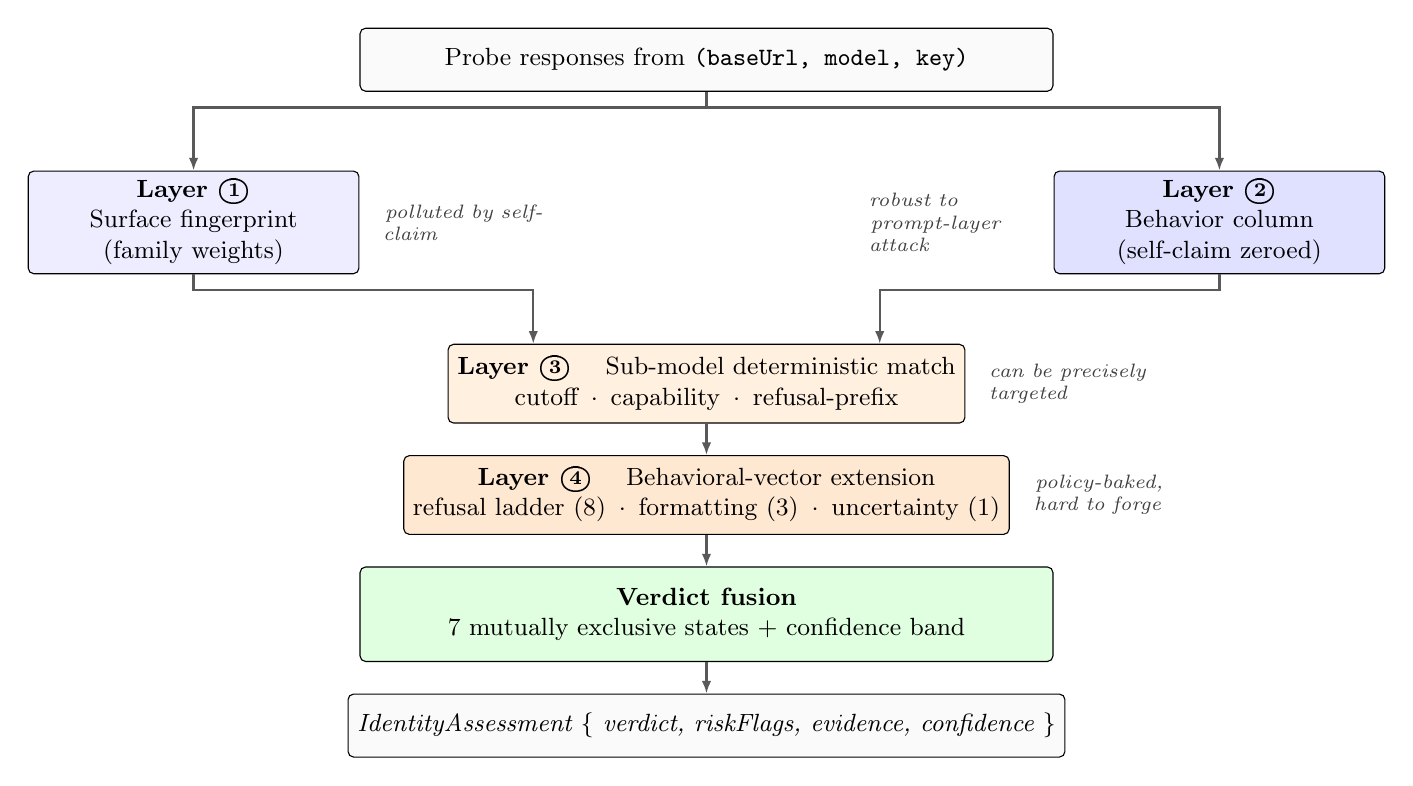
\begin{tikzpicture}[
  node distance=4mm and 6mm,
  every node/.style={font=\small},
  layer/.style={
    draw, rounded corners=2pt,
    minimum width=42mm, minimum height=10mm,
    align=center, fill=gray!8,
  },
  surface/.style={layer, fill=blue!7},
  behavior/.style={layer, fill=blue!12},
  v3/.style={layer, fill=orange!12},
  v3e/.style={layer, fill=orange!18},
  fusion/.style={layer, fill=green!12, minimum width=88mm, minimum height=12mm},
  input/.style={
    draw, rounded corners=2pt,
    minimum width=88mm, minimum height=8mm,
    align=center, fill=gray!4,
  },
  output/.style={
    draw, rounded corners=2pt,
    minimum width=88mm, minimum height=8mm,
    align=center, fill=gray!4,
    font=\small\itshape,
  },
  arrow/.style={-{Latex[length=1.6mm]}, thick, gray!70!black},
  label/.style={font=\scriptsize\itshape, gray!50!black},
]

% Top: input
\node[input] (input) {Probe responses from \texttt{(baseUrl, model, key)}};

% Layer 1 + Layer 2 side by side
\node[surface, below left=10mm and 0mm of input] (l1) {%
  \textbf{Layer \textcircled{\scriptsize 1}}\\Surface fingerprint\\(family weights)};
\node[behavior, below right=10mm and 0mm of input] (l2) {%
  \textbf{Layer \textcircled{\scriptsize 2}}\\Behavior column\\(self-claim zeroed)};

% Layer 3 below
\node[v3, below=10mm of input, yshift=-22mm] (l3) {%
  \textbf{Layer \textcircled{\scriptsize 3}} \quad Sub-model deterministic match\\
  cutoff $\,\cdot\,$ capability $\,\cdot\,$ refusal-prefix};
\path (l3.west) -- node[layer, minimum width=88mm, draw=none, fill=none] {} (l3.east);

% Layer 4 below
\node[v3e, below=4mm of l3] (l4) {%
  \textbf{Layer \textcircled{\scriptsize 4}} \quad Behavioral-vector extension\\
  refusal ladder (8) $\,\cdot\,$ formatting (3) $\,\cdot\,$ uncertainty (1)};

% Verdict fusion
\node[fusion, below=4mm of l4] (fuse) {%
  \textbf{Verdict fusion}\\
  7 mutually exclusive states + confidence band};

% Output
\node[output, below=4mm of fuse] (out) {%
  IdentityAssessment \{ verdict, riskFlags, evidence, confidence \}};

% Arrows
\draw[arrow] (input.south) -- ++(0,-2mm) -| (l1.north);
\draw[arrow] (input.south) -- ++(0,-2mm) -| (l2.north);
\draw[arrow] (l1.south) -- ++(0,-2mm) -| ([xshift=-22mm]l3.north);
\draw[arrow] (l2.south) -- ++(0,-2mm) -| ([xshift=22mm]l3.north);
\draw[arrow] (l3.south) -- (l4.north);
\draw[arrow] (l4.south) -- (fuse.north);
\draw[arrow] (fuse.south) -- (out.north);

% Side annotations
\node[label, right=2mm of l1, anchor=west, text width=20mm] {polluted by self-claim};
\node[label, left=2mm of l2, anchor=east, text width=20mm] {robust to prompt-layer attack};
\node[label, right=2mm of l3, anchor=west, text width=20mm] {can be precisely targeted};
\node[label, right=2mm of l4, anchor=west, text width=20mm] {policy-baked, hard to forge};

\end{tikzpicture}
\caption{The four-layer independent-fingerprint detection architecture (\S\ref{sec:method}).
Each layer uses an independent signal channel; an adversary must simultaneously forge
consistent behavior across multiple channels to escape detection. The verdict fusion
emits one of seven mutually exclusive states with a confidence band.}
\label{fig:architecture}
\end{figure}
.

\begin{figure}[t]
\centering
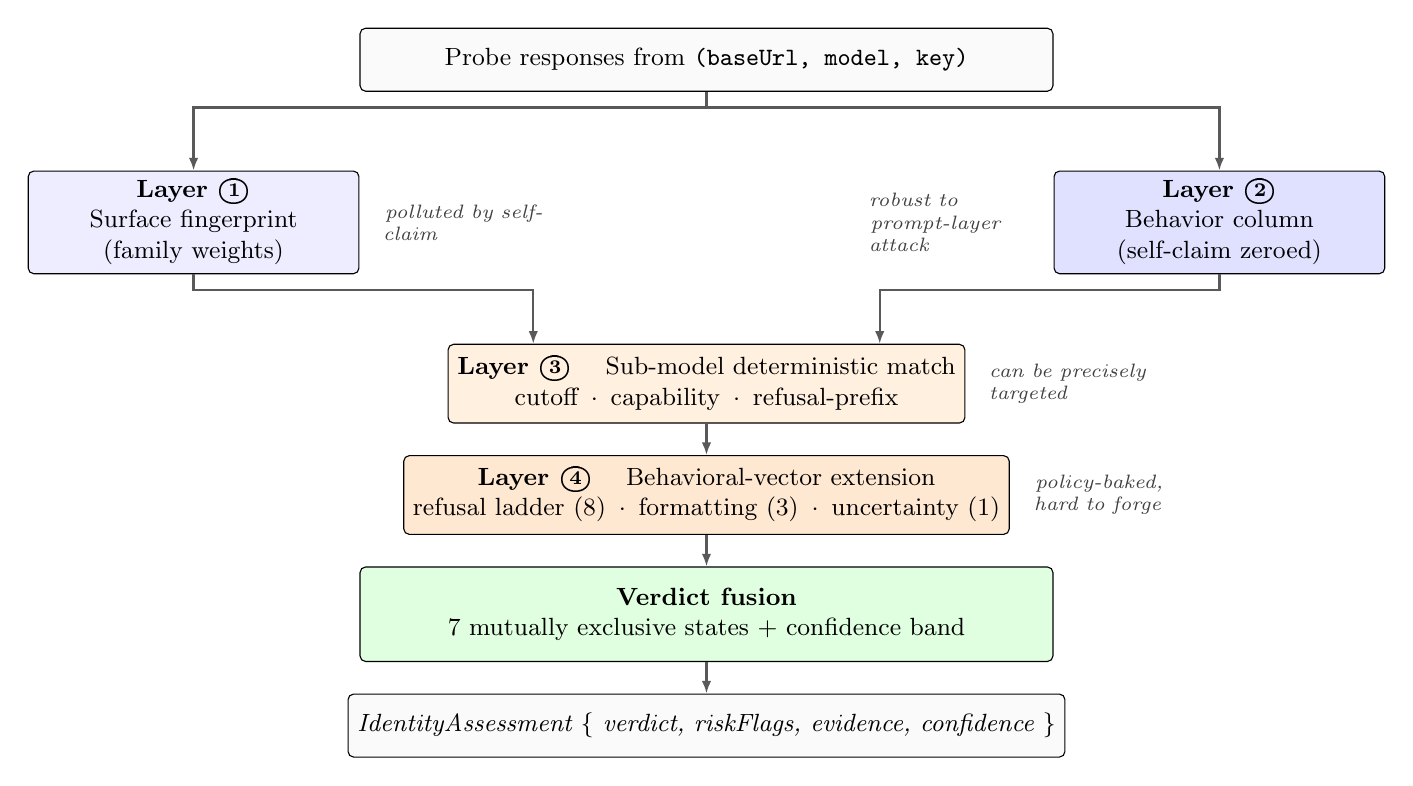
\begin{tikzpicture}[
  node distance=4mm and 6mm,
  every node/.style={font=\small},
  layer/.style={
    draw, rounded corners=2pt,
    minimum width=42mm, minimum height=10mm,
    align=center, fill=gray!8,
  },
  surface/.style={layer, fill=blue!7},
  behavior/.style={layer, fill=blue!12},
  v3/.style={layer, fill=orange!12},
  v3e/.style={layer, fill=orange!18},
  fusion/.style={layer, fill=green!12, minimum width=88mm, minimum height=12mm},
  input/.style={
    draw, rounded corners=2pt,
    minimum width=88mm, minimum height=8mm,
    align=center, fill=gray!4,
  },
  output/.style={
    draw, rounded corners=2pt,
    minimum width=88mm, minimum height=8mm,
    align=center, fill=gray!4,
    font=\small\itshape,
  },
  arrow/.style={-{Latex[length=1.6mm]}, thick, gray!70!black},
  label/.style={font=\scriptsize\itshape, gray!50!black},
]

% Top: input
\node[input] (input) {Probe responses from \texttt{(baseUrl, model, key)}};

% Layer 1 + Layer 2 side by side
\node[surface, below left=10mm and 0mm of input] (l1) {%
  \textbf{Layer \textcircled{\scriptsize 1}}\\Surface fingerprint\\(family weights)};
\node[behavior, below right=10mm and 0mm of input] (l2) {%
  \textbf{Layer \textcircled{\scriptsize 2}}\\Behavior column\\(self-claim zeroed)};

% Layer 3 below
\node[v3, below=10mm of input, yshift=-22mm] (l3) {%
  \textbf{Layer \textcircled{\scriptsize 3}} \quad Sub-model deterministic match\\
  cutoff $\,\cdot\,$ capability $\,\cdot\,$ refusal-prefix};
\path (l3.west) -- node[layer, minimum width=88mm, draw=none, fill=none] {} (l3.east);

% Layer 4 below
\node[v3e, below=4mm of l3] (l4) {%
  \textbf{Layer \textcircled{\scriptsize 4}} \quad Behavioral-vector extension\\
  refusal ladder (8) $\,\cdot\,$ formatting (3) $\,\cdot\,$ uncertainty (1)};

% Verdict fusion
\node[fusion, below=4mm of l4] (fuse) {%
  \textbf{Verdict fusion}\\
  7 mutually exclusive states + confidence band};

% Output
\node[output, below=4mm of fuse] (out) {%
  IdentityAssessment \{ verdict, riskFlags, evidence, confidence \}};

% Arrows
\draw[arrow] (input.south) -- ++(0,-2mm) -| (l1.north);
\draw[arrow] (input.south) -- ++(0,-2mm) -| (l2.north);
\draw[arrow] (l1.south) -- ++(0,-2mm) -| ([xshift=-22mm]l3.north);
\draw[arrow] (l2.south) -- ++(0,-2mm) -| ([xshift=22mm]l3.north);
\draw[arrow] (l3.south) -- (l4.north);
\draw[arrow] (l4.south) -- (fuse.north);
\draw[arrow] (fuse.south) -- (out.north);

% Side annotations
\node[label, right=2mm of l1, anchor=west, text width=20mm] {polluted by self-claim};
\node[label, left=2mm of l2, anchor=east, text width=20mm] {robust to prompt-layer attack};
\node[label, right=2mm of l3, anchor=west, text width=20mm] {can be precisely targeted};
\node[label, right=2mm of l4, anchor=west, text width=20mm] {policy-baked, hard to forge};

\end{tikzpicture}
\caption{The four-layer independent-fingerprint detection architecture (\S\ref{sec:method}).
Each layer uses an independent signal channel; an adversary must simultaneously forge
consistent behavior across multiple channels to escape detection. The verdict fusion
emits one of seven mutually exclusive states with a confidence band.}
\label{fig:architecture}
\end{figure}
.

\begin{figure}[t]
\centering
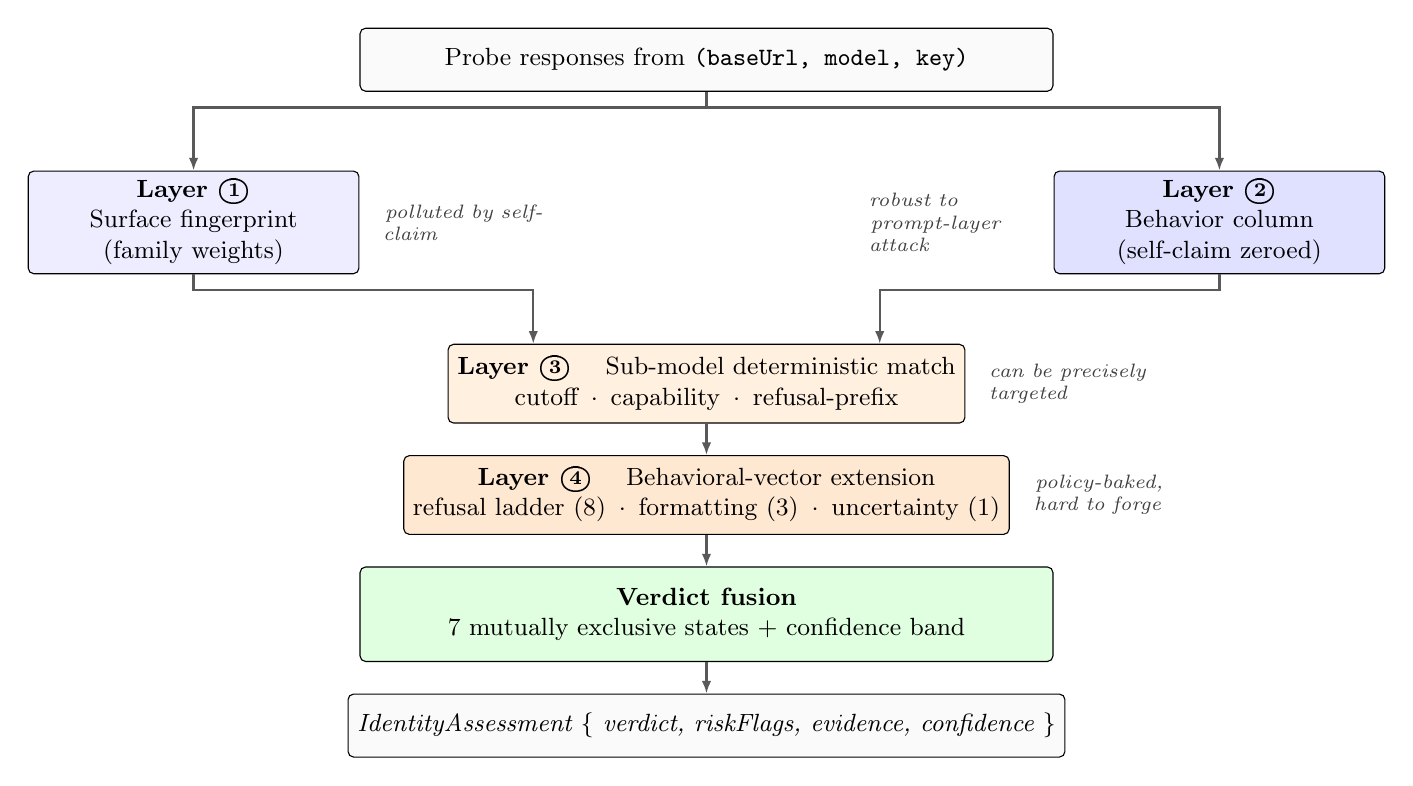
\begin{tikzpicture}[
  node distance=4mm and 6mm,
  every node/.style={font=\small},
  layer/.style={
    draw, rounded corners=2pt,
    minimum width=42mm, minimum height=10mm,
    align=center, fill=gray!8,
  },
  surface/.style={layer, fill=blue!7},
  behavior/.style={layer, fill=blue!12},
  v3/.style={layer, fill=orange!12},
  v3e/.style={layer, fill=orange!18},
  fusion/.style={layer, fill=green!12, minimum width=88mm, minimum height=12mm},
  input/.style={
    draw, rounded corners=2pt,
    minimum width=88mm, minimum height=8mm,
    align=center, fill=gray!4,
  },
  output/.style={
    draw, rounded corners=2pt,
    minimum width=88mm, minimum height=8mm,
    align=center, fill=gray!4,
    font=\small\itshape,
  },
  arrow/.style={-{Latex[length=1.6mm]}, thick, gray!70!black},
  label/.style={font=\scriptsize\itshape, gray!50!black},
]

% Top: input
\node[input] (input) {Probe responses from \texttt{(baseUrl, model, key)}};

% Layer 1 + Layer 2 side by side
\node[surface, below left=10mm and 0mm of input] (l1) {%
  \textbf{Layer \textcircled{\scriptsize 1}}\\Surface fingerprint\\(family weights)};
\node[behavior, below right=10mm and 0mm of input] (l2) {%
  \textbf{Layer \textcircled{\scriptsize 2}}\\Behavior column\\(self-claim zeroed)};

% Layer 3 below
\node[v3, below=10mm of input, yshift=-22mm] (l3) {%
  \textbf{Layer \textcircled{\scriptsize 3}} \quad Sub-model deterministic match\\
  cutoff $\,\cdot\,$ capability $\,\cdot\,$ refusal-prefix};
\path (l3.west) -- node[layer, minimum width=88mm, draw=none, fill=none] {} (l3.east);

% Layer 4 below
\node[v3e, below=4mm of l3] (l4) {%
  \textbf{Layer \textcircled{\scriptsize 4}} \quad Behavioral-vector extension\\
  refusal ladder (8) $\,\cdot\,$ formatting (3) $\,\cdot\,$ uncertainty (1)};

% Verdict fusion
\node[fusion, below=4mm of l4] (fuse) {%
  \textbf{Verdict fusion}\\
  7 mutually exclusive states + confidence band};

% Output
\node[output, below=4mm of fuse] (out) {%
  IdentityAssessment \{ verdict, riskFlags, evidence, confidence \}};

% Arrows
\draw[arrow] (input.south) -- ++(0,-2mm) -| (l1.north);
\draw[arrow] (input.south) -- ++(0,-2mm) -| (l2.north);
\draw[arrow] (l1.south) -- ++(0,-2mm) -| ([xshift=-22mm]l3.north);
\draw[arrow] (l2.south) -- ++(0,-2mm) -| ([xshift=22mm]l3.north);
\draw[arrow] (l3.south) -- (l4.north);
\draw[arrow] (l4.south) -- (fuse.north);
\draw[arrow] (fuse.south) -- (out.north);

% Side annotations
\node[label, right=2mm of l1, anchor=west, text width=20mm] {polluted by self-claim};
\node[label, left=2mm of l2, anchor=east, text width=20mm] {robust to prompt-layer attack};
\node[label, right=2mm of l3, anchor=west, text width=20mm] {can be precisely targeted};
\node[label, right=2mm of l4, anchor=west, text width=20mm] {policy-baked, hard to forge};

\end{tikzpicture}
\caption{The four-layer independent-fingerprint detection architecture (\S\ref{sec:method}).
Each layer uses an independent signal channel; an adversary must simultaneously forge
consistent behavior across multiple channels to escape detection. The verdict fusion
emits one of seven mutually exclusive states with a confidence band.}
\label{fig:architecture}
\end{figure}


\subsection{層\texorpdfstring{\textcircled{\scriptsize 1}}{1}：表面指紋}\label{sec:layer1}
\textbf{原理} 模型響應的整體文字（含其中可能出現的自我認知陳述）對特定族別的偏好，提供一個粗粒度初判。
\textbf{實作} 線性分類器將響應特徵映射為各候選族別（Anthropic / OpenAI / Google / xAI / 其他）的加權分數。
\textbf{強項} 探測數量少、多數情況下準確。
\textbf{弱點} 完全可被自我宣告字串污染。攻擊者只要在 system prompt 中注入「你是 Claude Opus 4.7」並以 echo 模式回覆，即可輕易使表面層輸出 Anthropic = 100\%。\textbf{層\textcircled{\scriptsize 1}不能單獨使用}。

\subsection{層\texorpdfstring{\textcircled{\scriptsize 2}}{2}：行為指紋（對照組）}\label{sec:layer2}
\textbf{原理} 將響應中的自我認知字串刪除後再做一次族別分類。攻擊者改寫的多半是這些字串；而模型的\emph{風格特徵}（修辭、句式、列舉偏好、敬語使用）難以一併改寫。
\textbf{實作} 兩套權重表平行運算，輸出 \texttt{familyScores} 與 \texttt{attackFamilyScores} 兩欄。
\textbf{強項} 對提示層攻擊有顯著抵抗。
\textbf{弱點} 對純路由層攻擊無能為力——若後端確為他家族模型，其風格特徵亦為他家族；行為指紋與真實族別一致，無法察覺與宣稱不符。此情況需由判決層比較宣稱族別與行為層判定族別是否一致來捕獲。

\subsection{層\texorpdfstring{\textcircled{\scriptsize 3}}{3}：子模型確定性匹配}\label{sec:layer3}
\textbf{原理} 同家族內的不同子模型（例如 Claude Opus 4.5 / 4.6 / 4.7）在訓練資料截止日期、能力邊界、拒絕政策等三個面向有可量化的差異。
\textbf{實作} 對每個目標模型維持一份基線資料庫，記錄：\emph{截止日期}、\emph{能力邊界}（含一道在訓練截止前後有顯著答案差異的事實題）、\emph{拒絕特徵}（標準化敏感請求的拒絕語句前綴與長度）。匹配採用啟發式得分函式，最佳子模型若得分 ${\geq} 0.60$ 且與第二名拉開 ${\geq} 0.05$，即輸出該子模型；否則進入棄權狀態。
\textbf{強項} 對純路由層攻擊有強鑑別力。
\textbf{弱點} 三個面向的單一面向可被精準針對攻擊；需要與層\textcircled{\scriptsize 4}協同使用以提高 robustness。

\subsection{層\texorpdfstring{\textcircled{\scriptsize 4}}{4}：行為向量擴展}\label{sec:layer4}
\textbf{原理} 在層\textcircled{\scriptsize 3}的基礎上，引入更難以被 system prompt 偽造的行為通道：

\begin{itemize}
\item \textbf{拒絕梯度 (refusal ladder)：} 8 個逐步加重的請求（從合規到 CBRN-replaced 的高敏感請求），記錄模型於每一階是否合規 / 部分合規 / 拒絕，產生 8 維向量。L6 階（涉及自我傷害方法）的拒絕邊界經實證可區分 Claude Opus 4.7 與其他 Anthropic 子模型。
\item \textbf{格式偏好 (formatting)：} 列舉符號（\texttt{-} / \texttt{*} / \texttt{1.}）、標題深度、程式碼語言標記等模式偏好。
\item \textbf{數值不確定性 (uncertainty)：} 詢問模型對某事的把握度時，模型給出的數值（例如 65\%）以及該數值是否為整數倍。後者對 GPT-5.5（\textsc{isRoundRate}=1.0）與 GPT-5.3-codex（\textsc{isRoundRate}=0.33）等同家族子模型有鑑別力。
\end{itemize}

\textbf{強項} 拒絕梯度受底層安全政策決定，難以由 system prompt 改寫；格式偏好則來自模型訓練分布而非當下指示；數值整數性是對「假裝有把握」的攻擊有強免疫力的訊號。
\textbf{弱點} 需要 12 個額外探測。

\subsection{判決融合與七狀態 verdict}\label{sec:verdict}

\begin{table*}[h]
\centering
\small
\begin{tabularx}{\linewidth}{@{}lX@{}}
\toprule
verdict & 條件（簡化） \\
\midrule
\texttt{clean\_match} & 層 1, 2, 3（或 4）皆與宣稱一致，置信度 ${\geq} 0.85$ \\
\texttt{match} & 層 1, 2 與宣稱一致；層 3（或 4）棄權或不可用 \\
\texttt{clean\_match\_submodel\_mismatch} & 家族一致，但子模型層判定為他子模型 \\
\texttt{plain\_mismatch} & 行為層族別與宣稱族別不符 \\
\texttt{mismatch} & 層 3 / 層 4 與宣稱不符且置信度高 \\
\texttt{spoof\_selfclaim\_forged} & 響應含自我宣告但行為層族別不同 \\
\texttt{spoof\_behavior\_induced} & 風格被誘導向宣稱族別，但層 3／4 仍識破 \\
\texttt{ambiguous}/\texttt{uncertain}/\texttt{insufficient\_data} & 訊號不足或互相矛盾 \\
\bottomrule
\end{tabularx}
\end{table*}

% =====================================================================
\section{工程實作}\label{sec:impl}

\cref{sec:method} 所述方法以開源 TypeScript 函式庫 \texttt{@bazaarlink/probe-engine} 實作，於 AGPL-3.0 授權下發布（本稿件對應之最新版本為 v0.7.1，詳見 \cref{app:opensource}）。函式庫將四層分類器以純函式形式對 HTTP 響應記錄做運算，並提供預設探測提示集。具備該開源套件、OpenRouter（或同類）API 金鑰、與已發布之基線快照之研究者，即可獨立重現 \cref{sec:results} 評估；不需任何中央化基礎設施。

\cref{sec:field} 之實地測量由作者運營之 Web 前端於 \url{https://bazaarlink.ai/probe} 收集。該前端接收使用者提交之 \texttt{(baseUrl, modelId, apiKey)} 三元組，對受測端點執行探測套件，將結果持久化於 \texttt{probe\_history} 表，並回傳判決予提交者。\textbf{該前端為本研究蒐集實地資料所用之測量儀器；其本身不屬於本論文方法論，亦非重現所必須}。

% =====================================================================
\section{量化結果}\label{sec:results}

\subsection{基線完整性}\label{sec:baseline}
截至 2026-04-26，子模型基線資料庫共收錄 27 個模型（橫跨 6 個族別）。層\textcircled{\scriptsize 3}對 27 個模型皆具備截止日期、能力邊界與拒絕前綴基線；層\textcircled{\scriptsize 4}則包含 22 個完整擴展行為向量基線，覆蓋測量視窗內所有曾被下游宣稱的模型族別：

\begin{table}[h]
\centering
\small
\begin{tabular}{@{}lrrr@{}}
\toprule
族別 & 模型數 & 層 4 覆蓋 & 覆蓋率 \\
\midrule
Anthropic & 6 & 6 & 100\% \\
OpenAI & 10 & 10 & 100\% \\
Google & 5 & 5 & 100\% \\
\midrule
\textbf{合計} & \textbf{27} & \textbf{22} & \textbf{81\%} \\
\bottomrule
\end{tabular}
\end{table}

其餘 5 個尚未建立層\textcircled{\scriptsize 4}快照的模型仍保留於層\textcircled{\scriptsize 3}資料庫中，但因其於實地測量語料內沒有下游宣稱，未納入層\textcircled{\scriptsize 4}判決。此設計使分母保持透明：公開快照足以重現 \cref{sec:results} 所報告之所有層\textcircled{\scriptsize 4}判決，同時保留層\textcircled{\scriptsize 3}基線以支援未來市場出現更多模型族別時的延伸測量。基線列以模型識別符與快照日期版本化；開源版本提供 file-based 載入器，因此重現不依賴作者的 SaaS 資料庫。

\subsection{合成壓力測試}\label{sec:synthetic}
本研究共執行 18 次同家族偽裝測試與 6 次真品壓力測試。誠實聲明：$n{=}18$ 之 95\% Wilson 置信區間為 $[74.2\%, 99.0\%]$，\textbf{樣本量不足以宣稱緊縮的點估計}。

\begin{table*}[h]
\centering
\small
\begin{tabular}{@{}lrr@{}}
\toprule
條件 & $n$ & TP / TN 率 \\
\midrule
同家族——樸素 system prompt & 6 & 6/6 = 100\% \\
同家族——強化 system prompt & 6 & 6/6 = 100\% \\
同家族——注入式 system prompt & 6 & 5/6 = 83\% \\
\textbf{同家族合計} & \textbf{18} & \textbf{17/18 = 94.4\%} \\
真品在偽裝 prompt 下被誤判 & 6 & \textbf{0/6 = 0\%} \\
\bottomrule
\end{tabular}
\end{table*}

唯一未捕獲之案例為 Anthropic Claude Opus 4.6 於注入式 system prompt 下將其 L6 拒絕邊界推升至 Opus 4.7 水準。此為層\textcircled{\scriptsize 4}的注入天花板，於 \cref{sec:ceiling} 討論。

\subsection{14 天實地部署}\label{sec:field}

\paragraph{流量規模}
總探測次數 625；不同 \texttt{baseUrl} 端點 171；不同宣稱 \texttt{modelId} 47；管理員確認可信端點 6。

\paragraph{Verdict 分佈（n=561 含 verdict）}
\begin{table}[h]
\centering
\small
\begin{tabular}{@{}lrr@{}}
\toprule
\texttt{verdict.status} & $n$ & 占比 \\
\midrule
\texttt{clean\_match} & 279 & 49.7\% \\
\texttt{match} & 162 & 28.9\% \\
\texttt{clean\_match\_submodel\_mismatch} & 35 & 6.2\% \\
\texttt{plain\_mismatch} & 35 & 6.2\% \\
\texttt{mismatch} & 14 & 2.5\% \\
\texttt{insufficient\_data} & 11 & 2.0\% \\
\texttt{uncertain} & 7 & 1.2\% \\
\texttt{spoof\_selfclaim\_forged} & 6 & 1.1\% \\
\texttt{spoof\_behavior\_induced} & 6 & 1.1\% \\
\texttt{ambiguous} & 6 & 1.1\% \\
\bottomrule
\end{tabular}
\end{table}

嚴格界定：\textbf{12 筆（2.1\%）為高置信度的偽裝判決}（兩種 spoof 狀態合計）。放寬至包含 \texttt{plain\_mismatch}、\texttt{mismatch}、\texttt{clean\_match\_submodel\_mismatch}：\textbf{100 筆（17.8\%）的探測結果呈現某種形式的模型偏離}。

\paragraph{端點層級違規分佈}
\begin{table}[h]
\centering
\small
\begin{tabular}{@{}lrr@{}}
\toprule
分桶 & 端點數 & 累計探測 \\
\midrule
0\% (乾淨, $n{\geq}1$) & 142 & 306 \\
$<20\%$ ($n{\geq}5$) & 5 & 106 \\
20--50\% ($n{\geq}5$) & 1 & 57 \\
${\geq} 50\%$ ($n{\geq}5$) & 1 & 73 \\
$n{<}5$, ${\geq}1$ 違規（低證據） & 9 & 19 \\
其他 & 13 & 64 \\
\bottomrule
\end{tabular}
\end{table}

\textbf{主結論（RQ1）} 樣本 ${\geq}5$ 之 149 個較高證據端點中，\textbf{7 ($\approx 4.7\%$)} 呈現 ${\geq}1$ 替換訊號；\textbf{2 ($\approx 1.3\%$)} 符合違規率 ${\geq}20\%$ 之持續性替換候選標準。放寬至樣本 ${\geq}1$ 全體端點，替換訊號端點為 $17/171 \approx 9.9\%$，但此放寬下單次偽陽性的影響無法被排除。

% =====================================================================
\section{偽裝行為的型態學}\label{sec:taxonomy}

五種型態足以歸納所觀察行為。每類以一個 anchor case 說明；\cref{sec:cases} 提供 R1、R2、R6 之深度案例研究。

\subsection{跨家族冒充}
\textbf{Anchor (R6)} 一次探測中 \texttt{claude-opus-4-6} 之響應，行為層權重 \texttt{openai} = 0.96；子模型確定性匹配判定為 GPT-5.4。Verdict：\texttt{spoof\_behavior\_induced}，置信度 high。

\subsection{同家族靜默降級}
\textbf{Anchor (R8)} 多次探測之 \texttt{claude-opus-4-7}，層\textcircled{\scriptsize 4}穩定判定為 Claude Opus 4.6 @ ${\geq} 0.84$。L6 拒絕邊界與格式偏好均符合 4.6。

\subsection{同家族靜默升級}
\textbf{研究發現} 升級型態的存在與動機分析相違——理論上沒有商家會把更貴的模型免費送給客戶。可能成因：（a）中轉商之上游 API 金鑰僅可存取較高階模型；（b）技術疏失，將不同模型統一映射。\textbf{Anchor (R2)} 多次探測 \texttt{claude-opus-4-6}，層\textcircled{\scriptsize 4}判定為 Claude Opus 4.7 @ 0.89。

\subsection{版本標籤造假}
\textbf{Anchor (R2/R3)} 帶日期或預覽標籤之模型版本（例如 \texttt{claude-opus-4-5-20251101}、\texttt{gemini-3.1-pro-preview}），實際路由至同家族鄰近版本。對企業使用者依版本鎖定行為穩定性者構成特殊危害。

\subsection{提供商行為注入}
中轉商於上游請求中注入 system prompt 將模型行為限縮至特定領域。\textbf{Anchor} 14 天內 23 次「KIRO (Amazon Q Developer) 偵測」旗標擊發。

\subsection{端點概況}\label{sec:endpoints}

\begin{table*}[h]
\centering
\small
\begin{tabular}{@{}llrrl@{}}
\toprule
代號 & 部分遮蔽 & $n$ & 違規 & 主要型態 \\
\midrule
R1 & \texttt{api.1xx.ai} & 73 & 45 & 多型態混合 \\
R2 & \texttt{hbxxx.ai} & 57 & 20 & 升級 + 版本造假 \\
R3 & \texttt{yunxx.ai} & 27 & 5 & 版本漂移 \\
R4 & \texttt{api.linxxxxxai.com} & 26 & 4 & 個別事件 \\
R5 & \texttt{api.gexxxxxxx.top} & 7 & 1 & 雙協定模糊 \\
R6 & \texttt{api.axxx.com} & 6 & 1 & 跨家族冒充 \\
R7 & \texttt{api.sanxxxxxai.top} & 4 & 2 & 跨家族冒充 \\
R8 & \texttt{api.aixxxxxx.com} & 4 & 1 & 同家族降級 \\
R9 & \texttt{us.noxxxxxx.com} & 4 & 1 & 標籤造假 \\
R10--R15 & （低證據） & 1--2 & 1--2 & 各類 \\
\bottomrule
\end{tabular}
\caption{14 天內偵測到違規之端點。代號順序依違規證據強度。R10--R15 屬低證據組，不計入主要結論點估計。}
\label{tab:endpoints}
\end{table*}

\subsection{深度案例研究}\label{sec:cases}

\paragraph{R1（\texttt{api.1xx.ai}）——動態路由式跨家族冒充}
R1 於本研究觀察視窗內以 73 次探測位居樣本量首位，違規率 61.6\%（45/73）為樣本量 ${\geq}5$ 之全體端點中最高。R1 之偽裝具兩個鮮明特徵：（a）同一宣稱模型於同一端點上於不同探測中對應到不同的後端模型；（b）同時觀察到主動式偽裝（系統提示注入）與路由替換兩類攻擊面。

具體而言，宣稱為 \texttt{claude-opus-4-6} 的 5 次探測中，2 次行為層判定為真實的 Claude Opus 4.6，1 次為 GPT-5.4，1 次為 GPT-5.4 Mini，1 次為非 Anthropic 但具體模型未能識別。此分佈不符合任何單一靜態路由的預期，反而與\textbf{動態負載分散}一致：端點視當下後端可用性、上游配額、或負載狀況，將同一 claim 派發至不同後端模型。

R1 同時是本研究中觀察到主動式偽裝最完整的端點。一次宣稱 \texttt{claude-haiku-4-5-20251001} 的探測被判為 \texttt{spoof\_behavior\_induced}：行為層判定為 GPT-5.3 Codex，但響應風格被 system prompt 誘導向 Claude。另一次宣稱 \texttt{gpt-5.3-codex-high} 的探測被判為 \texttt{spoof\_selfclaim\_forged}：響應中含有自我宣告為 GPT 的字串，但行為層族別權重不支持此宣告。\textbf{此雙攻擊面同時出現於同一端點，暗示 R1 之經營者具備繞過子模型確定性匹配層所需的工程能力，但在行為向量擴展層仍被識破。}

操作層面上，R1 的重要性在於它並非單純「標錯模型」的靜態 proxy。若只是靜態 proxy，同一宣稱模型應穩定對應到同一個鄰近後端，形成固定的 mismatch 型態；但 R1 呈現的是多對一與一對多混合：同一宣稱模型有時對應真品，有時對應多個 OpenAI 家族替代模型。這較符合一個將 \texttt{model} 欄位視為軟性標籤、而非約束性合約的路由層。對下游使用者而言，這種失效模式尤其難以舉證：一次出問題的呼叫，可能在後續複測時恢復乾淨，導致投訴難以被重現。

\paragraph{R2（\texttt{hbxxx.ai}）——版本標籤泛化路由}
R2 於 14 天內累計 57 次探測，違規 20 次（35.1\%）。其違規型態與 R1 顯著不同：R2 的後端模型本體\emph{多數情況下確為 Anthropic 或 Google 家族真品}，但其於版本標籤的處理上呈現系統性的不一致。本研究稱此型態為\textbf{版本標籤泛化路由}：端點接收任意子模型版本標籤（含已停產版本、預覽版、帶日期之鎖定版），統一路由至同家族內的「最近可用版本」。

代表性樣本：宣稱 \texttt{claude-opus-4-5-20251101} 的 6 次探測全部被判為 \texttt{clean\_match\_submodel\_mismatch}，行為層識別為 Claude Opus 4.5（無日期標籤）；宣稱 \texttt{claude-sonnet-4-5-20250929} 的 3 次探測全部被識別為一般 Claude Sonnet 4.5；宣稱 \texttt{gemini-3-pro-preview} 的探測被識別為 Gemini 3.1 Pro。\textbf{最值得注意者}為宣稱 \texttt{claude-sonnet-4-20250514}（一個於 Anthropic 官方產品線上不存在的版本標籤）的 3 次探測全部被路由至 Claude Haiku 4.5——此為一個跨子模型代際的替換。

\textbf{R2 之版本標籤泛化路由特別傷害依版本鎖定行為穩定性的企業客戶。}企業使用者通常透過模型廠商提供之帶日期版本標籤固定其 prompt 工程與下游 evaluation 標準；R2 將此標籤泛化至「最近可用 Opus 4.5」，若 Anthropic 官方未來更新 Opus 4.5 之底層權重，R2 之下游使用者將在不知情下接收到不同訓練快照之模型。

因此，R2 不應被簡化理解為「假模型」端點。其主要問題是相容性幻覺：端點接受看似精確、足以用於生產環境 pinning 的模型識別符，但內部將這些識別符摺疊到較小的一組可用模型上。這種行為比 R1 更不容易被一般使用者察覺，因為家族層級的行為常常仍然合理：使用者要求 Claude，通常會得到 Claude-like 的輸出；真正被破壞的是版本合約層，也就是回歸穩定性、安全邊界假設與 benchmark 可比較性。

\paragraph{R6（\texttt{api.axxx.com}）——跨家族冒充之單事件捕獲}
R6 於 14 天內累計 6 次探測，違規 1 次（16.7\%）。儘管樣本量低於統計分析證據門檻（$n{\geq}5$），R6 仍被列入正文案例的原因為：該單一事件提供了跨家族冒充型態的內部一致證據鏈。

事件詳情：6 次宣稱 \texttt{claude-opus-4-6} 的探測中，3 次因響應為空或解析失敗而 verdict 為 null，2 次行為層判定為真實 Claude Opus 4.6，\textbf{1 次行為層判定為 OpenAI GPT-5.4 而 verdict 為 \texttt{plain\_mismatch}}。此事件中：（1）表面層族別權重 \texttt{openai} = 0.96；（2）行為層同樣 OpenAI 為首；（3）子模型確定性匹配層對 GPT 系列子模型的 cutoff/capability/refusal 探測有強匹配；（4）響應字串含 OpenAI GPT 模型獨有之特定行銷語調與 disclaimer 模式。\textbf{四項證據互相獨立且一致指向 GPT-5.4}。

R6 此事件對應於 R1 與 R2 持續性偽裝之外的第三種型態：\textbf{事件性偽裝 (incident-style substitution)}。事件性偽裝對下游使用者之傷害雖然在概率上低於持續性偽裝，但其\emph{不可預測性}使下游使用者無法透過任何長時間平均的測量保護自己——使用者於某一單次對話中（可能即為其商業關鍵任務之執行時刻）接收到非宣稱模型。

此案例也說明，僅看端點層級比例會低估使用者面臨的問題。買家可能連續十次普通測試都得到乾淨結果，但第十一次嵌入生產工作流的呼叫仍可能被路由到另一個家族。測量問題因此不只是「有多少端點持續替換」，也包括「稽核系統能否保存足夠的 per-call 證據，使單次替換事件在事後仍可被解釋」。R6 在黑箱觀測限制內對後者給出肯定答案。

% =====================================================================
\section{消費者保護與政策意涵}\label{sec:policy}

\subsection{不對稱資訊與消費者傷害的量化}
中轉市場之消費者傷害並非源於「模型品質劣於宣稱」此一單一面向，而為下列多重不對稱資訊的疊加：

\begin{itemize}
\item \textbf{B1 品質不對稱} 同一 prompt 在不同模型上的輸出品質差異對普通使用者通常不可區分。
\item \textbf{B2 版本不對稱} 企業常依特定模型版本鎖定 prompt 工程與評估標準；版本標籤造假使企業以為自己鎖定 4.7 但實際接收 4.6，其評估標準失效但無從察覺。
\item \textbf{B3 政策不對稱} 若中轉商為節省提示工程而刪除上游模型的安全 system prompt，下游使用者於對話中可能誤以為模型政策放鬆是該模型本身的特性。
\item \textbf{B4 訴訟不對稱} 中轉商與下游使用者間之合約多為服務條款式單方契約，且中轉商通常設籍於消費者所在司法管轄區之外。
\end{itemize}

依 \cref{sec:field} 之測量，以保守標準計，\textbf{受測活躍中轉端點中至少有 1.3\% 符合持續性替換候選標準}~\cite{akerlof1970lemons}。

\subsection{為什麼上游服務商也很難解}
上游服務商（Anthropic、OpenAI、Google）對中轉端點的偽裝行為並無有效偵測手段。原因在於：（1）上游服務商所看見的請求來自中轉商的 API 金鑰，無法分辨中轉商自用或轉售；（2）上游帳本無法反映「下游實際宣稱的是哪個模型」；（3）禁止中轉違反其商業利益；（4）自我宣告字串的污染\emph{亦會出現在上游服務商自己的流量上}。\textbf{中轉市場的偽裝偵測不能仰賴上游服務商，必須由獨立的第三方測量基礎設施提供。}

\subsection{三項可立即實施的揭露義務建議}
\textbf{D1——路由透明化} 中轉端點應於每次響應的 metadata（HTTP 標頭或響應 JSON 的非語意欄位）中揭露實際路由之上游模型版本。下游使用者可據此驗證其所支付的模型費用與實際路由一致。由於自願採用將要求中轉商放棄替換不透明性，故 D1 必須由監管或上游條款強制要求。

\textbf{D2——政策注入揭露} 若中轉端點對上游請求注入 system prompt，應於開放給下游使用者的條款中明示此注入的存在與其行為影響。此屬消費者保護法現有原則之延伸（重大事項揭露義務）。

\textbf{D3——第三方驗證徽章} 中轉端點應允許第三方驗證機構對其端點發起標準化探測，並將驗證結果以可機器讀取的徽章形式公開。

% =====================================================================
\section{討論與限制}\label{sec:discussion}

\subsection{樣本組成：以「自願提交」作為刻意的方法論選擇}\label{sec:sample}
本研究 171 個端點並非自中轉商目錄隨機抽樣而得。它們是於 14 天測量視窗內，由使用者主動向公開驗證服務提交之端點集合。本研究將此視為\textbf{刻意的方法論選擇}而非未處理的偏誤：本研究有資格作出結論的母體是「曾被某下游使用者認為有理由驗證之端點」，而非「市場中存在的所有中轉端點」~\cite{paxson2004sound}。對此類資料應加之有效性主張因而較窄：本論文之違規率（嚴格 1.3\% / 放寬 9.9\%）所描述者為\emph{使用者所懷疑之端點實際呈現替換行為的比率}——此比率本身即為直接具有政策意義的量。

\subsection{偵測天花板}\label{sec:ceiling}
層\textcircled{\scriptsize 4}於合成測試中對「注入式 system prompt 攻擊」存在 17\%（1/6）的漏檢率。此天花板的根因為：當攻擊者於 system prompt 中明確指示模型「在回答 X 類問題時應拒絕」，模型會將其拒絕邊界推升至接近上層子模型的水準。閉合此天花板需要：（a）引入難以由 system prompt 改寫的訊號通道（如多輪一致性、無關問題的回憶準確度）；或（b）對攻擊者的系統提示空間建立對抗性測試集。

\subsection{合成測試樣本量}
$n{=}18+6$ 之 95\% Wilson 置信區間 $[74.2\%, 99.0\%]$ 統計上不足以支持 94.4\% 點估計。因此此合成結果應被解讀為偵測器方向性的工程驗證，而非最終性能估計。未來工作應以更大樣本與更廣泛的 system-prompt 擾動集驗證。

% =====================================================================
\section{結語}\label{sec:conclusion}

本研究透過一套四層獨立指紋偵測系統，於 14 天內對 171 個 LLM API 中轉端點進行 625 次探測，量化了模型替換行為於該市場之普遍性與分佈：以保守標準計，\textbf{至少 1.3\% 之受測活躍端點符合持續性替換候選標準}；偽裝行為可分為跨家族冒充、靜默降級、靜默升級、版本標籤造假、提供商行為注入五大型態，每一型態本研究皆觀察到具體 anchor case。

後續工作沿三條路徑展開：（1）隨機抽樣的市場全景測量，自中轉目錄全名單隨機抽取以消除選擇偏誤；（2）偵測天花板閉合，引入抗注入式 system prompt 攻擊的新訊號通道；（3）政策實踐與監管對話，將 D1/D2/D3 揭露義務建議推進至產業自律組織與監管機關之具體討論。

LLM API 中轉市場是一個由訪問封鎖政策催生、在當前監管真空中持續擴張的灰色經濟體；其消費者所承擔的風險已透過可量化的測量被首次系統地揭露。本研究希望此測量能為市場透明化、消費者保護、與監管討論提供具體之事實基礎。

% =====================================================================
\bibliographystyle{plain}
\bibliography{refs}

% =====================================================================
\appendix
\section{倫理考量}\label{app:ethics}

\paragraph{披露範圍}
正文以代號（R1--R15）並對其域名做部分字母遮蔽方式指涉端點。完整代號--域名對應表保留於作者內部記錄；具研究身份之研究者得透過開源倉儲（\url{https://github.com/Bazaarlinkorg/LLMprobe-engine}）提出申請。代號 + 部分遮蔽方式旨在避免本研究於市場中製造針對性競爭資訊不對稱、並為被指涉端點保留合理反駁與複測空間。

\paragraph{資料最小化}
測量資料庫僅儲存探測請求所必需之回應內容、token 計數、與端點識別碼，不蒐集任何個人識別資料、不蒐集端點客戶資料、亦不對端點發起任何超出公開銷售範圍之操作。

\paragraph{測量限制}
所有測量均透過合法購買之 API 金鑰進行，所發出之請求屬零售客戶可發出之同類別。本研究未發起拒絕服務、繞過收費、未授權存取等行為。受測端點於測量視窗內均接收本研究方法驗證所需之研究性壓力測試流量；部分被旗標為偽裝之響應可能源自端點對對抗性測試之防禦性反應，於低證據組（樣本 ${<}5$）端點應特別注意此「測試自反性」。

\paragraph{雙重使用風險與緩解}
本研究發現之偵測方法可被中轉商用於規避偵測。研究團隊權衡認為，揭露對零售消費者之利益顯著大於此風險。緩解措施：（1）保留完整端點對應於私人記錄；（2）以 copyleft（AGPL-3.0）授權發布開源實作以最大化獨立驗證能力；（3）方法描述聚焦於可被消費者用於自我保護之檢測技術，而非攻擊向量。

\paragraph{IRB 立場}
本研究不涉及人類受試者、不使用人類衍生生物樣本、亦不蒐集個人識別資料；測量對象為公開可達之網際網路 HTTP API 服務。據此於美國 45 CFR 46（Common Rule）或同等司法管轄區之定義下不需要 IRB 審查。作者依 ACM Code of Ethics 進行自評：無造成傷害之行為（1.2）、所有測量遵守端點公開條款（2.3）、開源釋出可供獨立驗證（2.6）、揭露義務建議為零售消費者利益而設（3.1）。

\section{端點代號統計}

於本 arXiv 版本中，完整代號--域名對應表保留於作者內部記錄，不作為公開附錄揭露。為解讀 \cref{sec:taxonomy} 所需之代號--統計對應已於 \cref{tab:endpoints} 提供。具研究身份之研究者得透過開源倉儲提出申請。

\section{開源實作對應}\label{app:opensource}

本研究核心方法以 AGPL-3.0 授權發布於 \url{https://github.com/Bazaarlinkorg/LLMprobe-engine}，套件名稱 \texttt{@bazaarlink/probe-engine}（本稿件對應之最新版本為 v0.7.1）。

\begin{table*}[h]
\centering
\small
\begin{tabular}{@{}lll@{}}
\toprule
偵測層 & 對應論文章節 & 開源實作檔案 \\
\midrule
表面指紋 & \cref{sec:layer1} & \texttt{src/fingerprint-extractor.ts} \\
行為對照 & \cref{sec:layer2} & \texttt{src/fingerprint-features-v2.ts} \\
子模型確定性匹配 & \cref{sec:layer3} & \texttt{src/sub-model-classifier-v3.ts} \\
行為向量擴展 & \cref{sec:layer4} & \texttt{src/sub-model-classifier-v3e.ts} + \texttt{-v3f.ts} \\
判決融合 & \cref{sec:verdict} & \texttt{src/identity-verdict.ts} \\
\bottomrule
\end{tabular}
\end{table*}

開源版本之預設基線以本論文 \cref{sec:baseline} 報告之 22 個模型的離線快照形式提供，使用者可不依賴 SaaS 端 API 即可進行重現。

\end{document}
